\chapter{Deseño}

%Debe describirse como se realiza o Sistema, a división deste en diferentes compoñentes e a comunicación entre eles.
%Así mesmo, determinarase o equipamento hardware e software necesario, xustificando a súa elección no caso de que non fose
%un requisito previo. Debe achegarse a un nivel suficiente de detalle que permita comprender a totalidade da estrutura do
%produto desenvolvido, utilizando no posible representacións gráficas.
Neste capítulo, explicaremos  os diferentes compoñentes que forman o sistema e as tecnoloxías empregadas, así como o proceso de desenvolvemento e implementación do mesmo.

\section{Compoñentes do sistema}\label{componentes}
No que respecta á arquitectura do sistema software desenvolvido, podemos identificar tres grandes compoñentes:
\begin{itemize}
    \item \textbf{Backend}. O backend da aplicación está formado polos diferentes scripts de Python que se encargan da descargar os datos, mediante a API, da web de COPERNICUS, da súa
    descompresión, o procesamento e o almacenamento no directorio apropiado para que se poida acceder a eles. Ademais, cun script de Python e o programa  \texttt{cron} de Ubuntu,
    definiremos unha tarefa a executarse automáticamente de forma mensual, de forma que, segundo teñamos dispoñibles novos datos, estes se descarguen e sexan accesibles ó usuario, para que
    teña sempre os datos máis recentes.
    \item \textbf{Middleware}. O middleware está formado polo servidor ERDDAP, que serve como unha capa intermedia entre o backend de Python e o frontend que verá o usuario final.
    Ademais, como comentamos na \hyperref[descricion]{introdución}, proporciona unha forma sinxela de acceder a datasets científicos en formatos de arquivos comúns, facilitando a
    xeración de gráficos e mapas. Coa implementación do noso propio servidor ERDDAP, poderemos almacenar nel, ademais dos datasets que xa veñen por defecto, uns cos nosos arquivos.
    \item \textbf{Frontend}. O frontend desenvolverase empregando HTML. Será un frontend sinxelo, de forma que, cando se acceda á aplicación na URL do servidor, o usuario
    vexa un mapa, acoutado á zona na que se realiza o estudo dos datos, e que poida elixir, por unha parte, un parámetro de entre os catro que se proporcionan, e un mes no rango de
    meses dispoñibles no dataset, actualizándose a información de forma dinámica.
\end{itemize}

\subsection{Backend}\label{backend}
Como xa comentamos, o backend da aplicación desenvolveuse en Python. A elección desta linguaxe de programación para este módulo é sinxela: é a linguaxe de programación máis axeitada
para traballar con grandes cantidades de datos. Ademais, é a linguaxe que ten maior compatibilidade con tódalas ferramentas que deberemos empregar para o procesado dos datos, o que
fai que sexa, practicamente, a única opción a ter en conta..

Así, o backend de Python divídese en catro scripts diferentes, cada un cunha funcionalidade determinada.

\subsubsection{Script principal e automatización}\label{app}
Por unha parte, temos o script principal, \texttt{app.py}. Este é o script dende o que se executa o programa. Nel, establécense os parámetros cos cales se executaran os módulos de
descarga e procesado dos arquivos, comprobando tamén a súa validez (como, por exemplo, que a data de inicio da busca sexa anterior á data de fin). Pódese executar tanto por liña de comandos
coma importando o arquivo e chamando á función.

Por outra parte, temos o script \texttt{auto.py}, o cal se encarga da automatización da descarga e procesado dos datos. Este será o script que executaremos con \texttt{cron} de forma mensual,
para manter os datasets actualizados. Este script obtén, a partir da data actual, as datas para as que realizaremos a busca, que serán entre o primeiro e último día do mes anterior. Desta
forma, executaremos o \textit{job} de \texttt{cron}, cunha frecuencia mensual, o día 10 de cada mes. Polo tanto, no caso da execución que se realizaría o día 10 de xaneiro de 2024, as
datas que se tomarían como referencia serían o 1 de decembro de 2023 como data de inicio, e o 31 de decembro de 2023 como data de fin. Decidiuse elixir o décimo día de cada mes para
a actualización dos datos debido a que, como se explica en \cite{s5pdata}, o procesado dos arquivos resultantes das medicións dos satélites ten unha latencia de 5 días. Así, asegurámonos
de que, cando se execute o script, tódolos arquivos que se deben ter en conta estarán dispoñibles.


\subsubsection{Script de descarga de datos}\label{descarga}
En segundo lugar, temos o script de descarga de datos. A súa función principal é \texttt{obtenArquivos}, que recibe como parámetros a area de interese da busca, as datas de inicio e de fin, o parámetro
para o que se realizará a busca e o directorio onde se almacenarán os arquivos. Se este directorio non existe, creao. A continuación, empregando a API de oData, realiza unha consulta para obter os
arquivos que se descargarán. Iterando por estes arquivos, obten o seu Id e o nome e, se estos non existen (tanto en formato zip, por estaren comprimidos, ou en formato zip, por estaren
descomprimidos), realiza a súa descarga, na función \texttt{descargaArquivo}. Posteriormente, descomprime o arquivo coa función \texttt{descomprimeArquivo}, os cales quedan dentro dunha carpeta co seu
nome. Por tanto, unha vez descargados e descomprimidos tódolos arquivos, móveos á carpeta principal e elimina tódalas subcarpetas.

No que respecta á función de descarga de arquivos, en primeiro lugar chama a unha función para obter o token de autorización preciso para descargar os datos. A continuación, crea a url para a
descarga e, mediante a libraría Session, descarga o arquivo, sempre que a resposta do servidor sexa positiva. Por outra parte, a función de descompresión dos arquivos comproba, en primeiro lugar,
que o ficheiro zip exista. Se é así, empregando a libraría zipfile, extrae os arquivos no directorio (imprimindo unha mensaxe de erro en caso de que o arquivo sexa inválido) e, unha vez feito, bórrao.

\subsubsection{Script de procesado de datos}\label{procesado}
Por último, temos o script que se encarga de procesar os datos. Nel, o módulo principal que empregamos é HARP que, como se explica en \ref{harp}, é unha ferramenta que permite a
lectura e procesado de datos de satélite. Neste módulo temos diferentes funcións de procesado, unha para cada un dos diferentes parámetros que se ofrecen na aplicación, xa que as
operacións deben personalizarse en función do parámetro. Así, establécese unha función xenérica que, en función do parámetro que se estea tratando, invoca a unha función ou outra e,
unha vez procesados tódolos arquivos e exportados os datos, elimina os arquivos que se descargaron, co obxectivo de optimizar o almacenamento do servidor (posto que estamos falando de
centenares de arquivos cada mes, con tamaños de entre 500MB e 1GB, os cales, unha vez procesados, non son de interese nin utilidade). Ademais, temos unha función denominada \texttt{obtenListaProdutos}
, para obter os arquivos a procesar.

Malia que cada unha das funcións de procesado son bastante semellantes, posto que realizan unha serie de operación similares entre elas, foi preciso particularizalas, xa que o nome das variables
que exportaremos difire en función do parámetro. Estas funcións reciben unha lista de arquivos a procesar e un directorio onde almacenar o arquivo final procesado. Empregando a función \texttt{
    import\_product} de harp, importamos os arquivos, realizando con eles unha serie de operacións para filtrar os datos segundo a súa calidade, como se indica nos diferentes manuais. Unha vez temos
tódolos produtos importados, realizamos unha serie de operacións, propias para cada produto, para quedarnos cos datos dunha zona e obter con eles unha cuadrícula; e unha serie de post-operacións,
globais a tódalas funcións, para realizar a agregación dos datos. A continuación, definimos o nome do arquivo a exportar (que segue o patrón parametro\_AAAAMM.nc), e gardámolo.

\subsection{Middleware}\label{middleware}
O middleware que empregamos será ERDDAP. Isto é un servidor de datos que proporciona unha forma simple e consistente de acceder e descargar múltiples datasets científicos, de diferentes fontes, nun
formato común, facilitando a elaboración de gráficos e mapas \cite{erddaphome}. Ademais, permite obter os datos en diversos formatos de arquivo, ademais de proporcionar funcións para estandarizar
as datas dos resultados ou proporcionar os mesmos en formatos de imaxe personalizados. A instalación de ERDDAP de referencia é aquela feita pola National Oceanic and Atmospheric Administration (
NOAA, Oficina Nacional de Administración Oceánica e Atmosférica) que, ademais de ter máis de 200 datasets, permite crear un servidor local para almacenar nel datos propios.

Para realizar esta instalación, só será necesario seguir os pasos que se indican en \cite{erddapsetup}, o que explicaremos máis detalladamente en \ref{desenvolvemento} e \ref{implementacion}. En
resumo, é preciso:
\begin{enumerate}
    \item Dispoñer dunha versión de Java 17.
    \item Configurar Tomcat.
    \item Descargar os arquivos de configuración de ERDDAP e realizar os cambios precisos para adaptalo ó sistema.
    \item Instalar o arquivo \texttt{.war} de ERDDAP.
    \item Iniciar o servidor e configurar os datasets que queremos que sexan visibles no mesmo.
\end{enumerate}

\subsection{Frontend}\label{frontend}
Para o frontend do proxecto, crearemos unha aplicación sinxela en Tomcat, empregando HTML. Facendo uso da funcionalidade que nos proporciona ERDDAP para xerar imaxes a partir dos datos, crearemos
unha interface na que teñamos, por unha parte, un mapa cos datos que queiramos visualizar e, por outra parte, dous selectores, un para seleccioanr o parámetro a consultar e outro para seleccionar
o mes e ano.

\section{Tecnoloxías empregadas}\label{tecnoloxias}
\subsection{Anaconda}\label{anaconda}

\subsection{HARP}\label{harp}

\section{Desenvolvemento do sistema}\label{desenvolvemento}
\subsection{Introdución}
Para poder comezar a desenvolver o sistema, primeiro foi preciso realizar unha introdución á detección mediante satélite de diferentes datos e ó funcionamento dos satélites de TROPOMI. Para isto,
foron de utilidade os seminario dispoñibles en \cite{ARSETformation}, de monitorización de alta resolución de $NO_2$ dende o espacio con TROPOMI; \cite{ARSETtools}, de ferramentas para analizar
datos de alta calidade de satélite; e \cite{ARSETaplications}, de aplicacións de observacións de satélites para a calidade do aire e a exposición á saúde. Neles, explícase o funcionamento básico dos
satélites e como miden e procesan os datos. Tamén se explican os diferentes niveis de datos que existen, como mencionamos na \hyperref[introducion]{introdución}. Dipoñemos de 4 niveis principais de
datos:
\begin{enumerate}
    \item \textbf{Nivel 0 (L0):} estes datos son datos crus, tal e como se obteñen das medicións do satélite, a máxima resolución.
    \item \textbf{Nivel 1 (L1):} son os datos de nivel L0, pero con referencias temporais e información dos sensores empregados para as medicións, coma coeficientes de calibración radiometrica e
    xeometrica.
    \item \textbf{Nivel 2 (L2):} os datos de nivel L1, pero con variables xeofísicas derivadas na mesma resolución e ubicación que os datos de nivel L1.
    \item \textbf{Nivel 3 (L3):} as variables obtidas dos datos de nivel L2, mapeadas en forma de cuadrículas espazo-temporais, completas e con consistencia.
\end{enumerate}

Empregar datos de nivel L3 ten diversas vantaxes:
\begin{itemize}
    \item Podemos dispoñer dun único arquivo por día (ou por mes, ou o período de tempo que nos interese). Polas características do satélite, o seu ciclo orbital é de 16 días, realizando 14 órbitas
    por día \cite{s5porbit}. Polo tanto, para dous días distintos, é posible que un arquivo non cubra a totalidade da área de interese. Ó realizar as operacións de agregación dos datos, aseguramos
    ter un único arquivo por día, facendo a manipulación dos datos moito máis sinxela.
    \item Datos dispostos en cuadrículas uniformes. Coa agregación dos datos, podemos crear tamén unha cuadrícula para os mesmos, dispoñéndoos de forma regular no mapa ou área que nos interese
    estudar.
    \item Arquivos de menor tamaño. Os arquivos de nivel L2 conteñen unha maior cantidade de datos, unha gran parte dos cales pode non ser relevante para o noso sistema. O seu procesamento a nivel
    L3 permite elimar estos datos e variables innecesarias, minguando o tamaño dos arquivos.
    \item Maior calidade nos datos. Nos diferentes manuais dos produtos, establécense diversos criterios de calidade asociados ós datos, que podemos empregar para descartar medicións de certas
    áreas pequenas do espazo en caso de que non teñan unha calidade suficiente. Desta forma, ó procesar os datos, podemos eliminar estas medicións de menor calidade e, como crearemos agregados por
    grandes períodos de tempo, evitaremos que queden vacíos.
\end{itemize}

O satélite SENTINEL 5P proporciona datos de seis parámetros moi relacionados coa contaminación atmosférica: ozono ($O_3$), tanto a columna troposférica (aquela que se forma en capas mais altas da
atmosfera) coma a columna total; dióxido de nitróxeno ($NO_2$), tanto a columna troposférica coma a total; dióxido de xofre ($SO_2$), a columna total; monóxido de carbono ($CO$), a columna total;
metano ($CH_4$), a columna total; e formaldehido ($HCHO$), a columna total. Tratar todos estes parámetros era difícil de abordar, polo que foi preciso descartar dous deles para non telos en conta.
Baseándonos na información dispoñible en \cite{airpollutants}, decidimos elixir os seguintes: $NO_2$, $CO$, $SO_2$ e $O_3$. Escolléronse estes parámetros por seren os que máis problemas de saúde
adoitan causar, ademais de por empregárense máis a miúdo nos diferentes mapas de contaminación.

\subsection{Descarga de datos}\label{appdescarga}
Unha vez decididos os parámetros, podemos comezar coa descarga dos datos. Para isto, no Dataspace Copernicus temos dispoñibles múltiples APIs que podemos empregar para acceder e descargar os datos
. Estas APIs poden ser de tres tipos: \textit{Catalogue APIs}, que permiten buscar no catálogo de produtos dispoñibles e descargar os arquivos; \textit{Streamlined Data Access (EDA) APIs}, que
permiten obter datos de observación terrestre (EO) xunto con ferramentas de procesamento e análise; e outras APIs, que permiten, por exemplo, o acceso a datos EO empregando \textit{buckets} de S3.
No noso caso, elixiremos unha API do primeiro tipo, xa que é preciso poder buscar e filtrar os produtos para descargar aqueles que nos interesen.

Empregaremos a API de OData, que está baseada en APIs REST e permite, empregando mensaxes HTTP sinxelas, publicar e editar recursos identificados con URLs. A documentación completa da API atópase
en \cite{odata}. En xeral, unha query OData contén a URL base xunto cunha serie de opcións, entre as que se atopan: \textit{filter}, \textit{orderBy}, \textit{top}, \textit{skip}, \textit{count} e \textit{expand}.
Dentro da opción de \textit{filter}, podemos filtrar por:
\begin{enumerate}
    \item \textbf{Nome do produto:} filter=Name. Buscando un produto específico polo seu nome.
    \item \textbf{Colección de produtos:} filter=Collection/Name. Buscar produtos dunha colección concreta (SENTINEL-1, SENTINEL-2, SENTINEL-3, SENTINEL-5P, SENTINEL-6 ou SENTINEL-1-RTC).
    \item \textbf{Data de publicación:} filter=PublicationDate. Filtrando entre un intervalo de datas, que pode incluír (con \texttt{ge} e \texttt{le}) ou non (con \texttt{gt} e \texttt{lt}) as datas que se
    empreguen.
    \item \textbf{Data de detección:} filter=ContentDate/Start / filter=ContentDate/End. Filtrando pola data de detección dos datos.
    \item \textbf{Área xeográfica:} filter=OData.CSC.Intersects(area=geography'SRID=4326;). Pódense filtrar os datos para elixir aqueles que crucen cun punto (\texttt{POINT(x,y)}) ou con polígono (\texttt{POLYGON()},
    cunha lista de puntos).
\end{enumerate}

Por outra parte, existen as seguintes opcións, que deben ir separadas dos filtros e entre elas empregando o símbolo $\$$:
\begin{itemize}
    \item \textbf{orderBy}: para ordenar de forma descendente (\texttt{desc}) ou ascendente (\texttt{asc}), que é a opción por defecto. Pódese filtrar por \textit{ContentDate/Start}, \textit{ContentDate/End},
    \textit{PublicationDate} ou \textit{ModificationDate}.
    \item \textbf{top}: para limitar o número máximo de ítems que devolverá a query. Por defecto é 20, e pode establecerse como un número enteiro entre 0 e 1000.
    \item \textbf{skip}: permite saltar un certo número de resultados para, por exemplo, poder paxinar en caso de que a query obteña moitos resultados. O valor por defecto é 0, e pode tomar un
    valor entre 0 e 1000.
    \item \textbf{count}: para obter o número exacto de produtos que coincidan coa query. Por defecto, está establecida a \texttt{False}, deshabilitada.
    \item \textbf{expand}: permite ver os metadatos completos de cada un dos resultados que obtivo a query. Acepta como argumentos \textit{Attributes} ou \textit{Assests}.
\end{itemize}

Para realizar a busca dos produtos, unicamente é preciso empregar unha libraría que nos permita facer peticións HTTP. Neste caso, elixiuse a libraría \texttt{requests} de Python, xa que permite
realizar estas peticións dunha forma moi sinxela. A URL base dende a que obteremos os datos é \texttt{https://catalogue.dataspace. copernicus.eu/odata/v1/Products}, engadiremos os seguintes filtros:
\begin{itemize}
    \item \textbf{Área xeográfica:} limitaremos a busca á Península Ibérica, para o que definiremos o seguinte polígono: \texttt{POLYGON((-9.647785 35.912135,-9.647785 44.230843,4.916224 44.230843,
        4.916224 35.912135,-9.647785\break 35.912135))}.
    Esta área é a que se mostra na imaxe \ref{areainterese}
    \begin{figure}
        \centerline{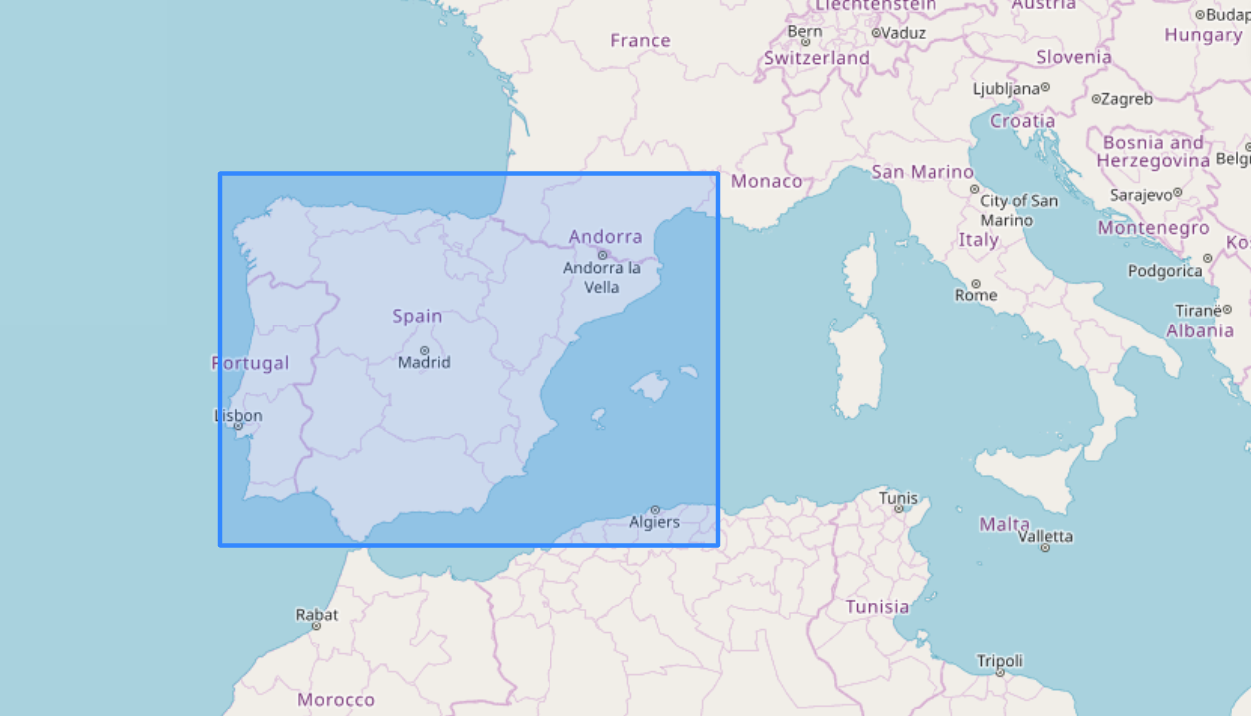
\includegraphics[width=10cm]{figuras/area.png}}
        \caption{Area de interese sobre a que se realiza a busca.}
        \label{areainterese}
    \end{figure}
    \item \textbf{Colección de produtos:} filtramos os produtos da colección \texttt{SENTINEL-5P}.
    \item \textbf{Nome de produto:} empregamos o filtro \texttt{contains(Name, 'S5P\_OFFL\_\{parametro\}')}, para obter os produtos do parámetro que nos interese.
    \item \textbf{Data de detección:} coas datas que se lle pasan á función dende o módulo principal da aplicación, filtramos en base á data de detección dos datos xa que, como comentamos en \ref{app}, os
    datos tardan varios días en publicarse dende que se miden.
    \item Aplicamos ademais a opción \texttt{top} para obter un número maior de resultados, que estableceremos a 100. Isto débese a que temos, de media, dous produtos por cada día que se busca e,
    no noso caso, ó facer buscas mensuais, o número de arquivos que se descargan será en torno a 60, moi superior ó límite de 20 que establece por defecto a API.
\end{itemize}
Os resultados obtidos desta petición almacénanse nunha variable que se convertirá a un DataFrame de \texttt{pandas}, que contén, entre outros, o nome do arquivo, o seu identificador, a data de
detección e publicación ou a pegada xeográfica. Así, iremos iterando sobre o DataFrame para, empregando o Id do produto e o seu nome, descargar os diferentes arquivos.

Para poder descargar os produtos, é preciso xerar un token de autenticación, xa que é preciso estar rexistrado. O proceso de rexistro é moi sinxelo, e pode facerse dende a páxina principal de
COPERNICUS. No noso caso, decidiuse elixir o correo corporativo da universidade, xunto cun contrasinal xenérico. Foi preciso tamén crear unha función, \texttt{get\_keycloak}, que, recibindo como
parámetros o usuario e o contrasinal, devolve o token de acceso. É preciso ter en conta as limitacións e cuotas que se explican en \cite{copquotas}, onde se explica que cada token de acceso é válido
durante 10 minutos, podendo ter un máximo de 100 sesións activas simultaneamente. Por iso, foi preciso xerar o token de acceso na propia función de descarga, e non antes de realizar a mesma xa que,
desta forma, corríase o risco de que a sesión expirase antes de poder descargar tódolos arquivos, o cal provocaría un fallo.

Unha vez temos o token de autenticación, creamos un obxecto de tipo \texttt{Session}, no cal estableceremos, mediante o método \texttt{.headers.update()}, o token de autenticación. A continuación,
establecemos a url na que se atopa o arquivo, que será \texttt{https://catalogue.dataspace.copernicus.eu/odata/v1/Products({id})\break/\$value}, onde id é o identificador do produto que vamos
descargar. Antes de descargar o arquivo, debemos comprobar o código de estado de HTTP da resposta, para comprobar que todo sexa correcto. Desta forma, descargaremos o arquivo se o código de estado
é 200 (OK) ou 308 (Permanent redirect). Se o estado é dos tipos 30X, significa que precisamos accións adicionais para completar a petición, polo que volveremos a repetila. Se o estado é correcto,
escribiremos o contido do arquivo nun ficheiro .zip, no directorio que corresponda.

Inmediatamente despois de descargar o arquivo, temos que descomprimilo posto que, como vimos de comentar, é preciso descargalo en formato ZIP. Para isto, temos unha función moi sinxela, denominada
\texttt{descomprimeArquivo}, que comproba que o arquivo exista e emprega a libraría zipfile para extraelo, comprobando tamén que sexa un arquivo zip válido (capturando a excepción \textit{zipfile
.BadZipFile}). Unha vez descomprimido, eliminaremos o ficheiro zip, posto que xa non será necesario. Debemos ter en conta que o ficheiro final que queremos obter, en formato netCDF (ou .mc) non se
atopará directamente no directorio en que se extrae, senón que se atopa dentro dunha subcarpeta co nome do arquivo que acabamos de descargar. Por tanto, unha vez descargamos e descomprimimos
tódolos arquivos, deberemos mover os ficheiros .nc ó directorio de descarga, podendo eliminar posteriormente tódolos subdirectorios.


\subsection{Procesamento de datos}\label{appprocesa}
Como xa comentamos, para procesar os datos empregaremos, principalmente, HARP \ref{harp}, unha ferramenta de lectura e procesado de datos de satélite, que se pode empregar en Python de forma moi
sinxela. A idea básica é importar unha serie de produtos, ós cales se lles aplican unha serie de operacións e postoperacións para transformalos en arquivos en cuadrículas regulares, e
posteriormente exportalos. Así, deseñamos unha función xenérica \texttt{transformaL3}, que recibe a ruta onde están os arquivos a procesar e o tipo de produto dos mesmos, e a ruta onde se exportar
á o arquivo resultante. Así, podemos optimizar o código, realizando dende esta función a chamada a cada unha das funcións deseñadas para cada un dos parámetros. Unha vez se procesa o arquivo en
cuestión, eliminaranse tódolos arquivos que se empregaron nesta operación, para cumplir co requisito \hyperref[rnf2]{[RNF2]}.

A continuación, explicarase máis detalladamente o proceso de transformación de cada un dos produtos.

\subsubsection{Transformación dos datos de $CO$}
A función de procesado dos datos de monóxido de carbono recibe, ó igual que as demais, unha lista de arquivos e unha ruta onde almacenar os arquivos procesados. Con esta lista de arquivos, podemos
iterar sobre ela, de forma que importamos os arquivos de un en un. Isto faise así, e non todos de golpe, para que o proceso de importado sexa máis eficiente e previr fallos ó ter que importar
numerosos arquivos simultáneamente. Así, empregamos a función \texttt{import\_products} de HARP, a cal nos devolve un produto de HARP que engadiremos a unha lista. Esta función pode recibir unha
serie de operacións que se aplicarán ós arquivos á hora de importalos. A lista das posibles operacións que se poden empregar en HARP atópase en \cite{HARPdoc}. No caso do monóxido de carbono, temos as
seguintes operacións:
\begin{enumerate}
    \item \texttt{\textbf{CO\_column\_number\_density\_validity\>5}}0 : con isto, filtramos os datos en base á calidade dos mesmos. Segundo as indicacións do manual de producto de CO (\cite{COmanual}),
    recoméndase ignorar os datos cun valor qa\_value menor que 0.5. Porén, como se explica en \cite{HARPCO}, a variable qa\_value é mapeada como CO\_column\_number\_density\_validity.
    \item \texttt{\textbf{derive(CO\_column\_number\_density [Pmolec/cm2]}}: a operación derive serve para cambiar o tipo de datos ou unidade dunha variable. Neste caso, cambiaremos o valor da
    columna de monóxido de carbono (que no arquivo orixinal se denomina carbonmonoxide\_total\_column) a petamoléculas por centímetro cadrado, xa que esta vén en moles por metro cadrado, para
    traballar con valores numéricos máis pequenos.
    \item \texttt{\textbf{keep(latitude, longitude, latitude\_bounds, longitude\_bounds, \break CO\_column\_number\_density)}}: con esta operación, indicamos que queremos incluír estas variables no
    produto.
\end{enumerate}

Unha vez importamos tódolos produtos, empregaremos a función \texttt{execute\_\break operations} para realizar operacións sobre os mesmos. Ó pasar unha lista de produtos á función, estes agruparanse
despois de realizar as operacións sobre os mesmos. Neste caso, as operacións a realizar son:
\begin{enumerate}
    \item \texttt{\textbf{bin\_spatial(2001, 35, 0.005, 3001, -10, 0.005)}}: esta operación mapea tódalas observacións nunha cuadrícula espacial de latitude/lonxitude. Neste caso, creamos unha
    cuadrícula de 2001 puntos de alto, comezando no paralelo 35\textdegree, cun \textit{offset} de 0.005\textdegree; e 3001 puntos de ancho, comezando no meridiano -10\textdegree, cun \textit{offset}
    de 0.005.
    \item \texttt{\textbf{exclude(latitude\_bounds\_weight, longitude\_bounds\_weight, weight, latitude\_weight, longitude\_weight)}}: excluímos estas variables do produto final.
    \item \texttt{\textbf{derive(latitude\{latitude\})}} e  \texttt{\textbf{derive(longitude\{longitude\})}}: derivamos as coordenadas de latitude e lonxitude da nova cuadrícula.
\end{enumerate}

Por último, aplicamos unha serie de post-operacións, que definimos de forma global nunha variable, xa que serán as mesmas para tódolos produtos:
\begin{enumerate}
    \item \texttt{\textbf{bin()}}: realiza un promedio de tódalas variables do produto na dimensión temporal.
    \item \texttt{\textbf{squash(time, (latitude, longitude))}}: elimina a dimensión \textit{time} para unha lista de variables (neste caso, \textit{latitude} e \textit{longitude}).
\end{enumerate}

Unha vez temos o arquivo resultante, almacenámolo no directorio indicado. Para obter o nome do arquivo, seguiremos a expresión \texttt{CO\_AAAAMM}, onde AAAA é o ano e MM é o mes do arquivo que
exportamos. Isto obtémolo directamente do nome de calquera un dos arquivos que empregamos.

\subsubsection{Transformación dos datos de $NO_2$}
Neste caso, o proceso é igual ó anterior. Os nomes das variables mapeadas atópanse dispoñibles en \cite{HARPNO2}. As operacións que aplicamos ó importar os produtos son:
\begin{enumerate}
    \item \texttt{\textbf{tropospheric\_NO2\_column\_number\_density\_validity\>75}}: neste caso, o manual de dióxido de nitróxeno (\cite{NO2manual}) indícanos que debemos considerar os datos cun 
    valor de qa\_value maior a 0.75.
    \item \texttt{\textbf{derive(tropospheric\_NO2\_column\_number\_density [Pmolec/cm2])}}: derivamos a variable que orixinalmente se denomina nitrogendioxide\_tropospheric\_\break column das súas
    unidades orixinais ($mol/m^2$) a $Pmolec/cm^2$.
    \item \texttt{\textbf{keep(latitude, longitude, latitude\_bounds, longitude\_bounds,\break tropospheric\_NO2\_column\_number\_density)}}: incluímos as variables no produto.
\end{enumerate}

As operacións que se executan sobre os datos son:
\begin{enumerate}
    \item \texttt{\textbf{bin\_spatial(2001, 35, 0.005, 3001, -10, 0.005)}}: creamos unha cuadrícula de 2001 puntos de alto, comezando no paralelo 35\textdegree, cun \textit{offset} de 0.005\textdegree;
    \item e 3001 puntos de ancho, comezando no meridiano -10\textdegree, cun \textit{offset} de 0.005.
    \item \texttt{\textbf{exclude(latitude\_bounds\_weight, longitude\_bounds\_weight, weight, latitude\_weight, longitude\_weight)}}: excluímos estas variables do produto final.
    \item \texttt{\textbf{derive(latitude\{latitude\})}} e  \texttt{\textbf{derive(longitude\{longitude\})}}: derivamos as coordenadas de latitude e lonxitude da nova cuadrícula.
\end{enumerate}

Aplicamos como post-operacións as mesmas que no anterior caso. O arquivo resultante almacénase no directorio indicado, e o seu nome segue a expresión \texttt{NO2\_AAAAMM}, onde AAAA é o ano e MM é o
mes o arquivo que exportamos.

\subsubsection{Transformación dos datos de $O_3$}
Para os datos do ozono, aplicamos as seguintes operacións ó importar os produtos:
\begin{enumerate}
    \item \texttt{\textbf{O3\_column\_number\_density\_validity\>50}}: neste caso, o manual do ozono (\cite{O3manual}) indícanos que debemos considerar os datos cun
    valor de qa\_value maior que 0.5.
    \item \texttt{\textbf{derive(O3\_column\_number\_density [Pmolec/cm2])}}: derivamos a variable que orixinalmente se denomina ozone\_total\_vertical\_column das súas
    unidades orixinais ($mol/m^2$) a $Pmolec/cm^2$.
    \item \texttt{\textbf{keep(latitude, longitude, latitude\_bounds, longitude\_bounds,\break O3\_column\_number\_density)}}: incluímos as variables no produto.
\end{enumerate}

Unha vez importados, executamos as seguintes operacións:
\begin{enumerate}
    \item \texttt{\textbf{bin\_spatial(2001, 35, 0.005, 3001, -10, 0.005)}}: creamos unha cuadrícula de 2001 puntos de alto, comezando no paralelo 35\textdegree, cun \textit{offset} de 0.005\textdegree;
    \item e 3001 puntos de ancho, comezando no meridiano -10\textdegree, cun \textit{offset} de 0.005.
    \item \texttt{\textbf{exclude(latitude\_bounds\_weight, longitude\_bounds\_weight, weight, latitude\_weight, longitude\_weight)}}: excluímos estas variables do produto final.
    \item \texttt{\textbf{derive(latitude\{latitude\})}} e  \texttt{\textbf{derive(longitude\{longitude\})}}: derivamos as coordenadas de latitude e lonxitude da nova cuadrícula.
\end{enumerate}

As post-operacións que se aplican son as mesmas que nos anteriores casos. O arquivo resultante almacénase no directorio indicado, e o seu nome segue a expresión \texttt{O3\_AAAAMM},
onde AAAA é o ano e MM é o mes o arquivo que exportamos.


\subsubsection{Transformación dos datos de $SO_2$}
Por último, para o caso do dióxido de xofre, seguimos a mesma lóxica que nos casos anteriores. Os nomes dos mapeos das variables atópanse en \cite{HARPSO2}. Aplicamos sobre os datos que importamos
as operacións:
\begin{enumerate}
    \item \texttt{\textbf{SO2\_column\_number\_density\_validity\>50}}: neste caso, o manual do dióxido de xofre (\cite{SO2manual}) indícanos que debemos considerar os datos cun
    valor de qa\_value maior que 0.5.
    \item \texttt{\textbf{derive(O3\_column\_number\_density [Pmolec/cm2])}}: derivamos a variable que orixinalmente se denomina sulfurdioxide\_total\_vertical\_column das súas
    unidades orixinais ($mol/m^2$) a $Pmolec/cm^2$.
    \item \texttt{\textbf{keep(latitude, longitude, latitude\_bounds, longitude\_bounds,\break SO2\_column\_number\_density)}}: incluímos as variables no produto.
\end{enumerate}

Sobre os datos importados, executamos as seguintes operacións:
\begin{enumerate}
    \item \texttt{\textbf{bin\_spatial(2001, 35, 0.005, 3001, -10, 0.005)}}: creamos unha cuadrícula de 2001 puntos de alto, comezando no paralelo 35\textdegree, cun \textit{offset} de 0.005\textdegree;
    \item e 3001 puntos de ancho, comezando no meridiano -10\textdegree, cun \textit{offset} de 0.005.
    \item \texttt{\textbf{exclude(latitude\_bounds\_weight, longitude\_bounds\_weight, weight, latitude\_weight, longitude\_weight)}}: excluímos estas variables do produto final.
    \item \texttt{\textbf{derive(latitude\{latitude\})}} e  \texttt{\textbf{derive(longitude\{longitude\})}}: derivamos as coordenadas de latitude e lonxitude da nova cuadrícula.
\end{enumerate}

As post-operacións que se aplican son as mesmas que nos anteriores casos. O arquivo resultante almacénase no directorio indicado, e o seu nome segue a expresión \texttt{SO2\_AAAAMM},
onde AAAA é o ano e MM é o mes o arquivo que exportamos.



\section{Implementación do sistema}\label{implementacion}
Unha vez comprobado que tódolos scripts funcionan correctamente, comezamos coa implementación do sistema deseñado na máquina de AWS que actuará como servidor. Os pasos a seguir serán configurar por
completo a máquina, instalando todo o software e paquetes precisos; instalar e configurar o servidor ERDDAP, para que lea os datos que se almacenan na máquina; e a implementación da interface á que
accederán os usuarios.

\subsection{Configuración da máquina de AWS}\label{aws}
Como se comentou anteriormente, empregaremos os Servizos Web de Amazon para configurar unha instancia de EC2 e empregala como servidor, instalando nela o servidor ERDDAP e procesando os datos.
Desta forma, facilítase que calquera usuario poida acceder dunha forma sinxela á aplicación dende a web.

A instancia que se elixiu é de tipo t3.xlarge, que dispón de 4 CPUs virtuais con 16 GiB de memoria, cunha AMI (Amazon Machine Image) de Ubuntu Jammy 22.04. A esta instancia acoplóuselle un volume de
almacenamento SSD de tipo gp2, con 250 GB de almacenamento, que permite 750 IOPS (\textit{Input/Output Operations per Second}). Ademais, obtívose unha dirección IP elástica, que se asociou á
máquina, de forma que garantizamos que a dirección IP non vai cambiar co tempo, e a aplicación será accesible sempre dende a mesma dirección. Esta dirección IP é a \texttt{13.53.65.240}. Todos estes recursos están
asignados á rexión eu-north-1 de Europa (Estocolmo), na zona de dispoñibilidade eu-north-1a.

Para poder acceder correctamente á máquina, debemos configurar as regras de entrada e saída do grupo de seguridade asociado á mesma. Neste caso, configuramos as regras de saída para permitir o tráfico
HTTP e HTTPS (portos 80 e 443) a tódolos destinos. No que ás regras de entrada se refire, permitimos tamén a entrada de todo o tráfico HTTP e HTTPS (portos 80 e 443); o tráfico SSH (porto 22), tamén
dende tódolos orixes, para poder conectarnos remotamente á máquina empregando unha terminal; e o tráfico TCP personalizado ó porto 8080, xa que é o porto que emprega Tomcat, onde estará o servidor
ERDDAP e a aplicación web.

Unha vez que temos a máquina funcionando, podemos instalar todo o software que será preciso para executar a aplicación. En primeiro lugar, instalamos Anaconda, unha distribución de Python que
simplifica a xestión e instalación de paquetes. A súa instalación é moi sinxela, pois só é preciso descargar o instalador para ubuntu e executalo, seguindo os pasos que indica. Unha vez instalado
Anaconda, crearásenos un entorno, que será dende o cal descarguemos os paquetes e executemos a aplicación. A lista de paquetes completa atópase no anexo \ref{manuais}. A continuación, debemos
instalar Java, na versión 17. Debemos empregar esta versión, ou superior, para poder configurar correctamente o servidor ERDDAP. Tamén deberemos instalar \texttt{nodejs}, xunto con \texttt{npm} (o
xestor de paquetes de nodejs), para poder executar a interface web.

O seguinte paso será instalar e configurar Tomcat. Debemos crear un usuario específico, \texttt{tomcat}, sen privilexios, para facer máis segura a instalación. Posteriormente, descargamos e
extraemos o \textit{core build} de Tomcat nun directorio (que, no noso caso, será \texttt{/opt/tomcat}), sobre o cal podemos conceder permisos ó usuario tomcat. Tamén debemos configurar os
administradores, para poder acceder ás páxinas de \textit{manager} e \textit{host-manager}. O último paso será crear un servizo en \texttt{systemd}, para que Tomcat poida executarse en segundo plano.
Nel, configuraremos as variables de entorno coma JAVA\_HOME, JAVA\_OPTS, CATALINA\_BASE e CATALINA\_HOME. Recargamos systemd e xa poderemos iniciar o servizo de Tomcat, o cal permitiremos que se
execute co inicio do sistema. Por último, debido a que Tomcat emprega o porto 8080, debemos permitir o tráfico nese porto tamén dende a máquina, empregando o comando \texttt{sudo ufw allow 8080}.

Neste punto, empregando os scripts que deseñamos en \ref{desenvolvemento}, executamos o módulo principal (\texttt{app.py}), decargando os datos para os catro parámetros que teremos dispoñibles para
un período de tempo razonable. No noso caso, decidimos descargar tódolos datos do ano 2023, dende xaneiro ata decembro. Posteriormente, este rango temporal poderase ampliar.

Finalmente, con Tomcat executándose e os datos dispoñibles no servidor, podemos comezar coa configuración do servidor ERDDAP.


\subsection{Configuración de servidor ERDDAP}\label{erddapconf}
Antes de comezar a instalar o servidor ERDDAP, debemos facer perquenos cambios nos arquivos de configuración de Tomcat. No arquivo \texttt{server.xml} (\textit{/opt/tomcat/conf/server.xml}),
debemos cambiar o valor do parámetro \texttt{connectionTimeout} dentro da etiqueta $<Connector>$ do porto 8080. No arquivo \texttt{context.xml} (\textit{opt/tomcat/conf/context.xml}), debemos
cambiar o valor de \texttt{cacheMaxSize} da etiqueta $<Resources>$ a 80000.

A continuacion, debemos descargar dende un repositorio de GitHub, proporcionado en \cite{erddapsetup}, un arquivo zip cos arquivos de configuración de ERDDAP. Debemos descomprimir este arquivo na 
carpeta de Tomcat, creando o directorio \textit{/opt/tomcat/content/erddap}. Dentro dos arquivos desta carpeta, atopamos \texttt{setup.xml}, o arquivo coa configuración que especifica como se
comporta o servidor ERDDAP. Nel, debemos cambiar: $<bigParentDirectory>$, que no noso caso establecemos como \textit{/home/ubuntu/erddap/}; $<baseURL$, que é a URL dende a que se accederá ó servidor;
$<emailEverythingTo>$, que é a dirección de correo á que se envían mensaxes de erro; e tódolos campos con etiquetas $<email*>$ e $<admin*$, con información relativa ó administrador do sistema (por
exemplo, $<adminIndividualName>$, co noso nome; $<adminCity>$, coa cidade; ou $<adminEmail>$, co noso email).

Con isto listo, podemos instalar o arquivo war de ERDDAP. Para isto, podemos descargalo directamente dende a URL que se indica en \cite{erddapsetup}, descargándoo directamente no directorio \textit{/opt/tomcat/webapps}.
Con isto, teríamos configurado xa o servidor ERDDAP cunha instalación básica, con tódolos datasets que veñen por defecto. Este está accesible na url \url{http://13.53.65.240:8080/erddap/index.html} .
Para poder incluír os nosos propios datasets, deberemos modificar o arquivo \textit{/opt/tomcat/content/erddap/datasets.xml}, seguindo os consellos que se indican en \cite{erddapdatasets}. Os
creadores de ERDDAP proporcionan, ademais, unha ferramenta denominada \texttt{GenerateDatasetsXml}, o cal permite facilitar este proceso.

Para cada datasets, crearemos unha etiqueta $<dataset>$, na cal configuraremos parámetros coma o \textit{type} (EDDGridFromNcFiles), o \textit{datasetId}, o seu estado (\textit{active=true} ou \textit{active=false}),
cada canto se recarga e se actualiza ($<reloadEveryNMinutes>$, que estableceremos a 10080 (7 días); e \break$<updateEveryNMillis>$, que será 60000 (1 minuto)), o directorio onde se atopan os
arquivos (no caso de, por exemplo, o monóxido de carbono, será \textit{/home/ubuntu/TFG/data/CO/}), ou a expresión regular no nome dos arquivos (que é \textit{.*\textbackslash.nc}) . Podemos
engadir atributos, coma o nome título do dataset, un resumo dos datos que ten ou as variables do mesmo. Tamén engadiremos tres \texttt{axisVariable}: unha para o tempo, que podemos derivar do nome
do arquivo, xa que este é unha expresión regular; a latitude, que se obtén directamente do arquivo; e a lonxitude, que tamén se obtén do arquivo. Por último, engadiremos unha \texttt{dataVariable}, que
será a variable que se mostrará no mapa. Engadirémoslle atributos coma o tipo de dato (\textit{double}), o nome, o valor mínimo e o valor máximo. A configuración completa do arquivo datasets.xml
está no anexo \ref{manuais}.


\subsection{Realización da interface}\label{interface}
Para crear a interface, crearemos unha aplicación nova en Tomcat, para illala do servidor ERDDAP. Crearemos unha nova carpeta no directorio \textit{/opt/tomcat/webapps}, denominada TROPOMIVisor.
Este será o nome da aplicación, que teremos que poñer na URL para acceder á mesma. Desta forma, a url para acceder á aplicación sería \url{http://13.53.65.240:8080/TROPOMIVisor/}
O deseño da interface será sinxelo, xa que ERDDAP permite acceder a un gráfico dos datos mediante unha URL específica. Por tanto
